\begin{figure}[p]
\centering
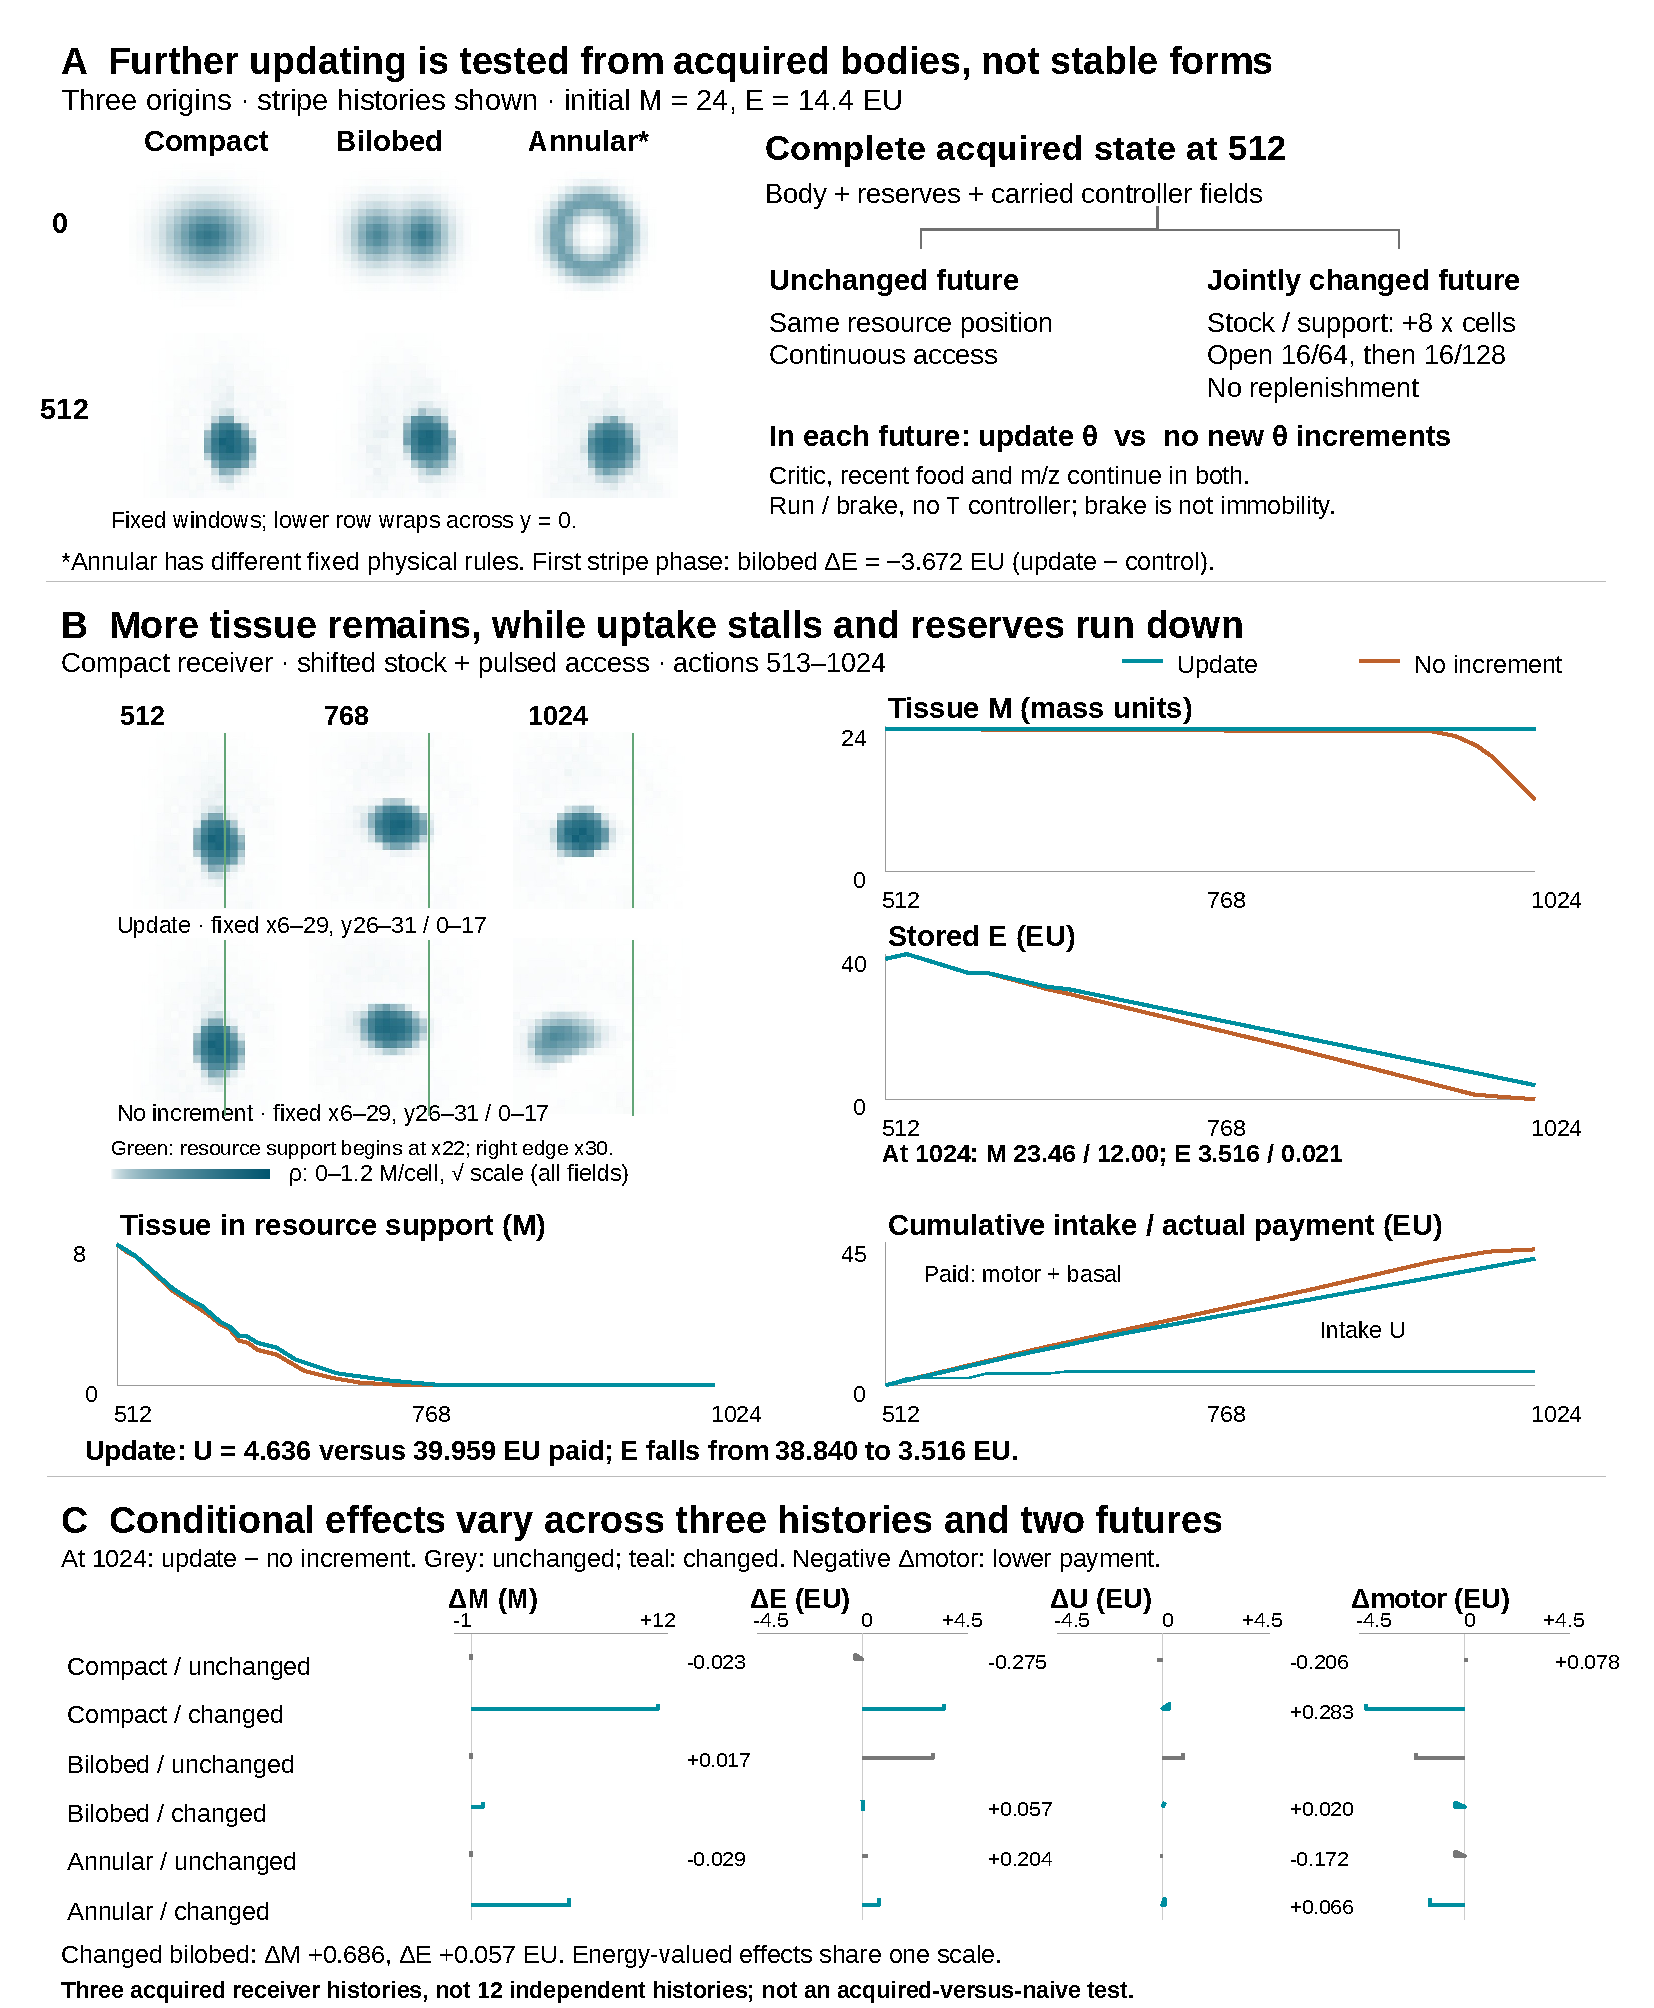
\includegraphics[width=0.90\linewidth]{figures/main/action_updating/adaptive_action_renewal.pdf}
\caption{\textbf{Continued action updating can retain tissue without sustaining substantial acquisition.}
\textbf{a,} Three structural origins and their acquired stripe states at step 512, shown in fixed original-coordinate windows; the lower window crosses the periodic $y$ boundary. Names denote origins, and the annular origin uses different fixed physical coefficients. Each acquired complete state supplies unchanged and jointly shifted/pulsed futures, each with or without further actor-logit increments. Other online processes continue; the run/brake controller has no interval $T$, and braking suppresses polarity readout rather than immobilizing tissue.
\textbf{b,} Compact origin under the changed future. Original-coordinate density windows, resource-support tissue and whole-body stock/receipt curves show that the larger retained mass coexists with very low late uptake and declining reserves. Green lines mark the resource support, not whether access is currently open. Actual payments combine motor and basal costs; energy lost with tissue is separate. Curves use archived per-action ledgers, rendered as simplified native polylines.
\textbf{c,} All six continuation contrasts (update minus no further increments). Energy-valued contrasts share one scale. The three acquired histories are not twelve independent histories. These conditional continuation effects do not measure acquired-versus-naive transfer benefit or establish sustained adaptation.}
\label{fig:action-renewal}
\end{figure}
